%%%%%%%%%%%%%%%%%%%%%%%%%%%%%%%%%%%%%%%%%
% Beamer Presentation
% LaTeX Template
% Version 1.0 (10/11/12)
%
% This template has been downloaded from:
% http://www.LaTeXTemplates.com
%
% License:
% CC BY-NC-SA 3.0 (http://creativecommons.org/licenses/by-nc-sa/3.0/)
%
%%%%%%%%%%%%%%%%%%%%%%%%%%%%%%%%%%%%%%%%%

%----------------------------------------------------------------------------------------
%	PACKAGES AND THEMES
%----------------------------------------------------------------------------------------

\documentclass{beamer}

\mode<presentation> {
\usetheme{CambridgeUS} % 
}

\usepackage{graphicx}
\usepackage{booktabs}
\usepackage[utf8]{inputenc}
\usepackage[portuguese]{babel}

%----------------------------------------------------------------------------------------
%	TITLE PAGE
%----------------------------------------------------------------------------------------

\title[Avanços da Engenharia Genética]{Avanços da Engenharia Genética}
\author{Rodrigo Magalhães dos Santos}
\institute[IPT]
{
Instituto de Pesquisas Tecnológicas \\ Universidade de São Paulo \\
\medskip
\textit{rmagalhaes85@gmail.com}
}
\date{16/04/2014}

\begin{document}

\begin{frame}
\titlepage
\end{frame}

\begin{frame}
\frametitle{Visão Geral}
\tableofcontents 
\end{frame}

%----------------------------------------------------------------------------------------
%	PRESENTATION SLIDES
%----------------------------------------------------------------------------------------

%------------------------------------------------
\section{Too Much Information} 
%------------------------------------------------

\begin{frame}
\huge{\centerline{Too Much Information}}
\normalsize{\centerline{(Muita Informação)}}
\end{frame}

\begin{frame}
\frametitle{Amniocentese}
\begin{itemize}
\item Permite analisar a informação genética do feto;
\item Avalia a ausência ou presença de falhas genéticas em larga-escala, como a cópia extra do cromossomo 21 (Síndrome de Down);
\item Baixo percentual de procura do exame, devido ao desconforto causado e à possibilidade de aborto espontâneo;
\end{itemize}
\end{frame}

\begin{frame}
\frametitle{Amniocentese}
\begin{itemize}
\item Não se trata de um exame de rotina. Só é recomendado em casos de maior risco de doenças genéticas;
\item Normalmente é realizado a pedido dos pais e não dos médicos;
\end{itemize}
\end{frame}

\begin{frame}
\frametitle{Amniocentese no Brasil}
\begin{itemize}
\item Ao contrário de outros países, no Brasil a lei não permite o aborto caso sejam encontrados defeitos genéticos como a Síndrome de Down;
\item Caso sejam encontrados problemas que representem incompatibilidade com a vida, um juíz pode decidir pela autorização do aborto;
\item Entretanto, mesmo nesses casos a autorização pode ser negada;
\end{itemize}
\end{frame}

\begin{frame}
\frametitle{Sequenciamento de DNA pré-natal}
\begin{itemize}
\item Recentemente, empresas lançaram um novo exame que coleta material genético do feto a partir do sangue da mãe;
\item O teste pode ser realizado em um estágio de gravidez mais precoce que a Amniocentese;
\item Estima-se que esse teste terá grande índice de adesão devido à simplicidade do procedimento (baixos riscos envolvidos na coleta de amostras de sangue);
\item Os resultados ainda não são tão precisos quanto os da Amniocentese;
\end{itemize}
\end{frame}

\begin{frame}
\frametitle{Argumentos em defesa do exame}
\begin{itemize}
\item A detecção da ausência de certos problemas reduziria a ansiedade dos pais;
\item A detecção de problemas precocemente permitirá aos pais se prepararem para a chegada de um filho com necessidades especiais;
\item Os médicos poderiam se preparar para prestar cuidados especiais logo após o nascimento da criança;
\end{itemize}
\end{frame}

\begin{frame}
\frametitle{Problemas decorrentes}
\begin{itemize}
\item A precisão dos resultados ainda precisa ser aprimorada;
\item Em algumas situações, o teste poderá simplesmente indicar alta \emph{probabilidade} do desenvolvimento de alguma doença. Nesse caso, o que fazer?
\end{itemize}
\end{frame}

\begin{frame}
\frametitle{Problemas éticos}
\begin{itemize}
\item Possibilidade de resgatar os aspectos mais nefastos da Eugenia;
\item Afinal, temos a sabedoria necessária para guiar nossa própria evolução?
\item Existem limites para a quantidade de informação que os pais deveriam ou gostaria de ter a respeito de seus filhos antes do nascimento?
\end{itemize}
\end{frame}

\begin{frame}
\frametitle{Problemas éticos}
\begin{itemize}
\item Supondo que fetos com Síndrome de Down passariam a ser abortados com frequência, o número de pessoas com a Síndrome diminuiria; 
\item Com isso, o mesmo ocorreria com o apoio a pesquisas na área, gerando grandes prejuízos aos futuros e atuais portadores da Síndrome;
\end{itemize}
\end{frame}

\begin{frame}
\frametitle{Problemas éticos}
\begin{itemize}
\item Certos defeitos genéticos não geram manifestações que prejudicam a vida do indíviduo. Como saber se este será o caso?
\item Exemplo hipotético: se um casal de portadores de nanismo desejarem ter um filho parecido com eles, seria considerado correto permitir o aborto de uma criança que não portasse nanismo?
\end{itemize}
\end{frame}

%------------------------------------------------

\section{DIY Chromosomes}

%------------------------------------------------

\begin{frame}
\huge{\centerline{DIY Chromosomes}}
\normalsize{\centerline{(Cromossomos "faça-você-mesmo")}}
\end{frame}

\begin{frame}
\frametitle{Biologia Sintética}
\begin{itemize}
\item Ramo que estuda a síntese de DNA em laboratório;
\item Nos transgênicos atuais, uma das técnicas consiste em retirar o gene de um organismo e inserir em outro;
\item Na biologia sintética, sequências de DNA são programadas do zero;
\end{itemize}
\end{frame}

\begin{frame}
\frametitle{Levedura}
\begin{itemize}
\item Fungo utilizado há milênios pela humanidade em processos de fermentação para a produção de pães, vinhos etc;
\item Já existem versões transgênicas da levedura usadas para a produção de insulina e drogas anti-malária;
\end{itemize}
\end{frame}

\begin{frame}
\frametitle{Levedura}
\begin{figure}
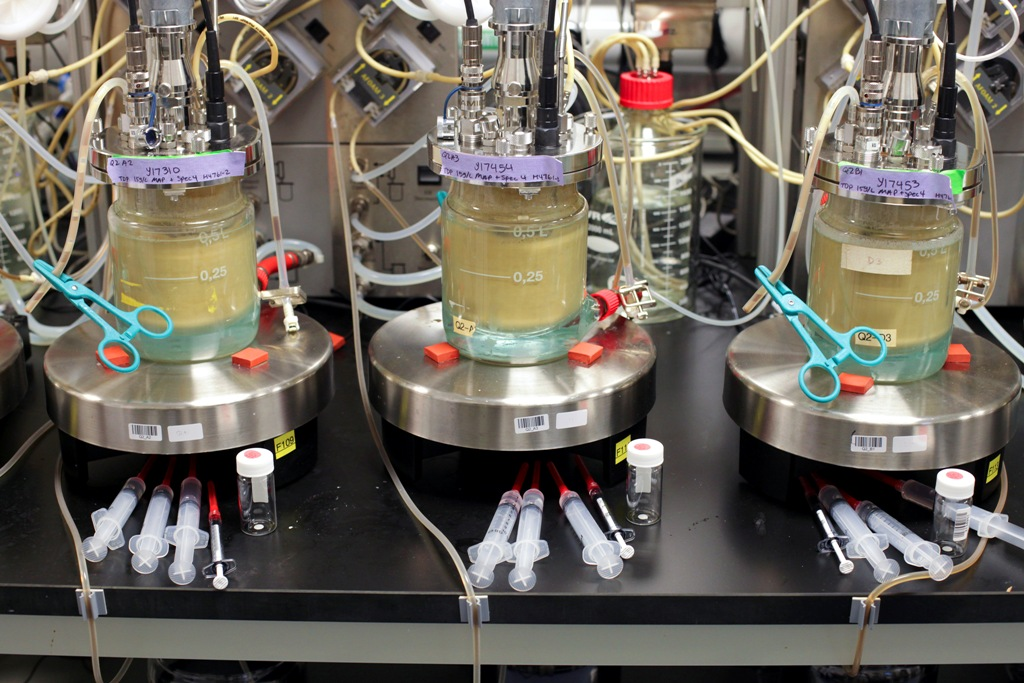
\includegraphics[scale=0.9]{Fermenters.jpg}
\caption{Fermentadores da empresa Amyris, com leveduras transgênicas usadas para produzir uma droga contra a malária (artemisina). Crédito: Jim Wilson/The New York Times}
\end{figure}
\end{frame}

\begin{frame}
\frametitle{Cromossomos sintéticos}
\begin{itemize}
\item Alguns grupos de cientistas já conseguiram sintetizar o DNA de vírus e bactérias (células \emph{procariontes});
\item Cientistas da Universidade Johns Hopkins sintetizaram um cromossomo completo de levedura;
\item Trata-se de um passo extremamente importante, já que foi a primeira vez que um grupo conseguiu sintetizar DNA de um microorganismo \emph{eucarionte};
\end{itemize}
\end{frame}

\begin{frame}
\frametitle{Células Procariontes x Células Eucariontes}
\begin{figure}
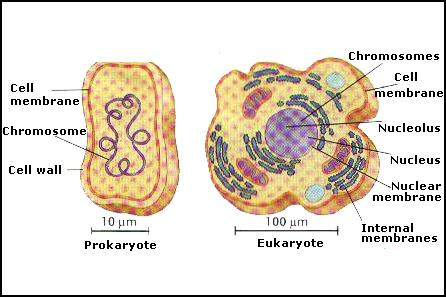
\includegraphics[scale=0.55]{prokaryotic-and-eukaryotic-cell-structures.jpeg}
\end{figure}
\end{frame}

\begin{frame}
\frametitle{Células Procariontes x Células Eucariontes}
\begin{itemize}
\item \textbf{Células Procariontes}: não possuem núcleo definido; estruturas simples;
\item \textbf{Células Eucariontes}: possuem núcleo bem definido para abrigar o DNA; possuem \emph{organelas}, pequenos "órgãos" com funções especializadas; 
\end{itemize}
\end{frame}

\begin{frame}
\frametitle{O que são Cromossomos?}
\begin{figure}
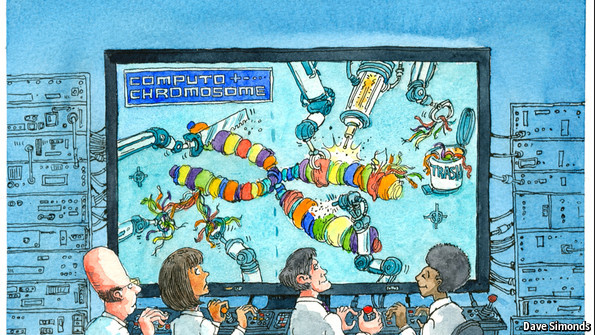
\includegraphics[scale=0.5]{students_chromosome.jpg}
\end{figure}
\end{frame}

\begin{frame}
\frametitle{O que são Cromossomos?}
\begin{figure}
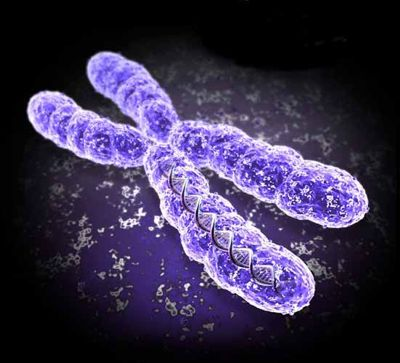
\includegraphics[scale=0.5]{chromosome2.jpg}
\end{figure}
\end{frame}

\begin{frame}
\frametitle{O que são Cromossomos?}
\begin{figure}
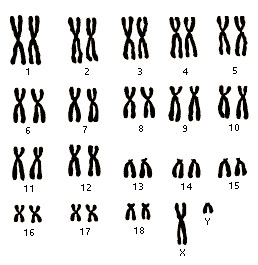
\includegraphics[scale=0.7]{human_chromosomes.jpg}
\end{figure}
\end{frame}

\begin{frame}
\frametitle{O que são Cromossomos?}
\begin{itemize}
\item Estruturas responsáveis por armazenar o DNA em pacotes compactos;
\item A quantidade de cromossomos varia dependendo da espécie;
\item Os humanos possuem 23 pares cromossomos. A Levedura possui 16 pares;
\end{itemize}
\end{frame}

\begin{frame}
\frametitle{Resultado da alteração do cromossomo pela equipe}
\begin{itemize}
\item Ao longo de anos, a equipe sintetizou em computador um dos cromossomos da levedura;
\item O cromossomo escolhido sofreu uma série de alterações, como remoção de alguns trechos e inserção de pontos para posterior "edição" do cromossomo;
\end{itemize}
\end{frame}

\begin{frame}
\frametitle{Resultado da alteração do cromossomo pela equipe}
\begin{itemize}
\item Por exemplo, foi inserido um ponto que permitira retirar novos trechos do cromossomo a partir da aplicação de enzimas;
\item A levedura criada artificialmente se comportou de maneira normal;
\end{itemize}
\end{frame}

%------------------------------------------------

%\begin{frame}
%\frametitle{O Protocolo IP no modelo de referência TCP/IP}
% \begin{figure}
% \includegraphics[width=0.6\linewidth]{ip-header-1.png}
% \caption{Fonte: http://www.thegeekstuff.com/2012/03/ip-protocol-header/}
% \end{figure}
%\end{frame}

%------------------------------------------------

\section{Referências}

%------------------------------------------------

\begin{frame}
\frametitle{Referências}
\footnotesize{
\begin{thebibliography}{9} 

\bibitem[B.C., 2012]{p1} Babycenter. (2012)
\newblock Amniocentese
\newblock \emph{Disponível em http://brasil.babycenter.com/a1500585/amniocentese}

\bibitem[Estadão, 2014]{p1} Estadão. (2014)
\newblock Cientistas criam cromossomo sintético para leveduras
\newblock \emph{Disponível em http://blogs.estadao.com.br/herton-escobar/cientistas-criam-cromossomo-sintetico-para-leveduras/}

\end{thebibliography}
}
\end{frame}

%------------------------------------------------

\begin{frame}
\Huge{\centerline{Dúvidas?}}
\end{frame}

%----------------------------------------------------------------------------------------

\begin{frame}
\Huge{\centerline{Fim}}
\end{frame}

%----------------------------------------------------------------------------------------

\end{document} 
